\documentclass[aspectratio=169]{beamer}


%%% PAQUETES  %%%
%%% PAQUETES  %%%


%%% TODONOTES y definición 2cm de margen para que no se solapen añadido colores comentarios
\setlength {\marginparwidth }{2cm} 
\usepackage{todonotes}
\usepackage[normalem]{ulem}

\usepackage[normalem]{ulem}

%%%%%%%%%%%%%%%%%%%%%%%%%%%%%%%%%%%%%%%%%%%%%%%%%%%%%%%%%%%%%%%%%%%%%%%%%%%%%%%%%

%%% Tildes y demás caracteres en español...
%\usepackage[latin1]{inputenc}
% o bien
\usepackage[utf8]{inputenc}

%%% Fuente Times...
\usepackage{times}

%%% Figuras en formato .png, .ps, pdf o eps
\usepackage{graphicx}
\usepackage{subfigure}
\DeclareGraphicsExtensions{.png,.eps,.ps,.pdf}

%%% Soporte graficos svg
\usepackage{svg}

%%% Formato y tipografía de URL, direcciones de correo...
\usepackage{url}
%\usepackage{hyperref}

%%% Sección para definir explícitamente la separación de sílabas al final de una línea:
\hyphenation{si-guien-do}

%%% Secciones etc. en castellano
\usepackage[spanish,es-tabla]{babel}

%%% Paquete para poner hipervinculos más finos \href
\usepackage{hyperref}

\hypersetup{
    colorlinks=true,
    linkcolor=black,
    filecolor=black,
    %%% Necesita su propia definicion de color
    citecolor=dimgray,  
    urlcolor=coolblack,
}



\usepackage{xcolor}

%%% Paquete para comentarios
\usepackage{verbatim}

% Definiciones colores extra
%% Ref: http://latexcolor.com/
	\definecolor{coolblack}{rgb}{0.0, 0.18, 0.39}
	\definecolor{dimgray}{rgb}{0.41, 0.41, 0.41}


%%% Paquete para usar simbolos y scripts de dibujado
\usepackage{tikz}
\def\checkmark{\tikz\fill[scale=0.4](0,.35) -- (.25,0) -- (1,.7) -- (.25,.15) -- cycle;} 
\usetikzlibrary{shapes,arrows}

% Define Block styles
\tikzstyle{decisionBL} = [diamond, draw, fill=blue!20,text width=10em, text badly centered, node distance=3cm, inner sep=0pt]
\tikzstyle{blockBL} = [rectangle, draw, fill=blue!20,text width=9em, text centered, rounded corners, minimum height=4em]
\tikzstyle{blockYL} = [rectangle, draw, fill=yellow!20, text width=9em, text centered, rounded corners, minimum height=4em]
\tikzstyle{blockGR} = [rectangle, draw, fill=green!20, text width=9em, text centered, rounded corners, minimum height=4em]
\tikzstyle{blockRD} = [rectangle, draw, fill=red!20, text width=9em, text centered, rounded corners, minimum height=4em]
\tikzstyle{blockWH} = [rectangle, draw, fill=white!20, text width=9em, text centered, rounded corners, minimum height=4em]
\tikzstyle{line} = [draw, -latex']
\tikzstyle{cloud} = [draw, ellipse,fill=red!20, node distance=4.5cm,minimum height=4em]

%%% Para usar ficheros tex de infografias Inkscape
\usepackage{pstricks}
%\definecolor{Azuloscuro-cisis}{RGB}{1,62,133}
\definecolor{Azulclaro-cisis}{RGB}{0,101,219}

\definecolor{LUCopper}{rgb}{0.8,0,0} %títulos slides
\definecolor{LUBlue}{rgb}{0.07, 0.04, 0.56}

\definecolor{LUPink}{rgb}{0.24,0.82,0.44}
\definecolor{LUGreen}{rgb}{0.24,0.82,0.44}
\definecolor{LUWhite}{rgb}{1,1,1} % fondo
%%% COMANDOS  %%%
%%% COMANDOS  %%%

%%% A cursiva  %%%
\newcommand{\cursiva}[1]{\em{#1}}


%%% Fuzzing en bonito  %%%
\newcommand{\fz}{\em fuzzing}

%%% Atajos estilo  %%%

\newcommand{\CLASSINPUTinnersidemargin}{18mm}
\newcommand{\CLASSINPUToutersidemargin}{12mm}
\newcommand{\CLASSINPUTtoptextmargin}{20mm}
\newcommand{\CLASSINPUTbottomtextmargin}{25mm}

\newcommand{\new}[1]{\textcolor{olive}{{#1}}}
%\newcommand{\old}[1]{\textcolor{purple}{{\sout{#1}}}}
\newcommand{\wip}[1]{\textcolor{blue}{{#1}}}
%\newcommand{\checkthis}[1]{\textcolor{orange}{{#1}}}
\newcommand{\diego}[1]{\textcolor{magenta}{{#1}}}
\newcommand{\vmodixit}[1]{\textcolor{teal}{{#1}}}

\newcommand{\old}[1]{\textcolor{purple}{{\sout{#1}}}}
\newcommand{\camino}[1]{\textcolor{olive}{{#1}}}
\newcommand{\fjrodl}[1]{\textcolor{blue}{{#1}}}
\newcommand{\checkthis}[1]{\textcolor{orange}{{#1}}}

%%% Entornos  %%%
\newcounter{definicion}
\newenvironment{definicion}[1]{%
    \refstepcounter{definicion}\par\medskip%
    \noindent \textbf{Definición~\thedefinicion. #1}.\ %
}{\medskip}

%%%% Soporte para el logo de ORCID
%\newcommand{\orcid}[1]{\href{https://orcid.org/#1}{\textcolor[HTML]{A6CE39}{\aiOrcid}}}



\title[{\fz} robots HPC]{\textbf{Fuzzing Robotic Software using HPC}\\
%\tiny \\
%\tiny y desacoplada para el uso de técnicas de {\fz} en HPC.\\
\small{\underline{Francisco Borja Garnelo Del Río}, Francisco J. Rodríguez Lera } \\
\small{Camino Fernández Llamas, Vicente Matellán Olivera} \\
\tiny{Universidad de León - 
Campus de Vegazana s/n, 24071 León (Spain)} \\
\tiny{infbgd01@estudiantes.unileon.es, \{fjrodl, cferll, vmato\}@unileon.es}
}

\titlecolor{LUWhite} % Choose between LUPink, LULBlue, LUIvory, LUGreen


\titleimage{\includegraphics[scale=0.55]{./img/conferencia.png}}

\author{Francisco B. Garnelo del Río (infbgd01@estudiantes.unileon.es)}

%\subtitle{\\ 
%\small{\underline{\\Francisco Borja Garnelo Del Río}, \\Francisco J. Rodríguez Lera,}\\ 
%\small{Camino Fernández Llamas, Vicente Matellán Olivera} \\
%\tiny{Universidad de León - Campus de Vegazana s/n, 24071 León (Spain)} \\
%\tiny{infbgd01@estudiantes.unileon.es, \{fjrodl, cferll, vmato\}@unileon.es}
%} 

\date{CISIS 2023}

\begin{document}
%\renewcommand{\contentsname}{Contenidos}
%\renewcommand{\figurename}{Figura}
%\renewcommand{\tablename}{Tabla}
%\renewcommand{\sectionname}{Sección}
%\renewcommand{\subsectionname}{Subsección}
%\renewcommand{\partname}{Parte}

\titleframe

\begin{frame}{Table of Contents}

\begin{enumerate}
\item Introduction
\begin{itemize}
    \item Goals and Hypotheses
    \item State of the art
\end{itemize}
\item Materials and Methods
\begin{itemize}
    \item Infrastructures
    \item Software
    \item Experiments
    \item Implemented cases
\end{itemize}
\item Results
\item Conclusions
\item Next steps
\end{enumerate}
 \end{frame}

 %% REF: Cajas https://texdoc.org/serve/tcolorbox.pdf/0

 % INTRODUCCION %%%%%%%%%%%%%%%%%%%%%%%%%%%%%%%%%%%%%%%%%%%%%%%%%
\section{Introduction}
%\frame{\sectionpage}
\begin{frame}{Introduction}

  
  
  \only<1>{

  %% TODO: Añadir Como abordamos el reto:
  %%% Dejar solo en 2 slide con items
\begin{tcolorbox}[drop shadow southeast,
enhanced,colback=blue!5!white,colframe=Azuloscuro-cisis]
\textbf{Fuzzing} is the automation of generating and testing malformed inputs in software in order to find unexpected behavior in the software.
\end{tcolorbox}

\begin{tcolorbox}[drop shadow southeast,
enhanced,colback=blue!5!white,colframe=Azuloscuro-cisis]
\textbf{Robotic systems} are systems that interact with their environment, including people, through the use of numerous sensors, actuators, and user interfaces to give intelligent services and information.
\end{tcolorbox}

\begin{tcolorbox}[drop shadow southeast,
enhanced,colback=blue!5!white,colframe=Azuloscuro-cisis]
\textbf{High Performance Computing (HPC)} is a technique that processes huge multidimensional information and solves complex problems at incredibly fast rates by using clusters of powerful processors operating in parallel.
\end{tcolorbox}

}

\end{frame}

%%% Goals and Hypotheses %%%%%%%%%%%%%%%
\subsection{Goals and Hypotheses}
%\frame{\subsectionpage}
\begin{frame}{Introduction - Goals and Hypotheses}
  \only<1>{

\begin{tcolorbox}[drop shadow southeast,
enhanced,colback=blue!5!white,colframe=Azuloscuro-cisis,title=Research question ]
What are the implications of using HPC systems when fuzzing ROS applications?
\end{tcolorbox}

This question arises from the following hypothesis and questions: 

\begin{tcolorbox}[drop shadow southeast,
enhanced,colback=blue!5!white,colframe=Azuloscuro-cisis]

\begin{itemize}
    \item \textbf{H1:} Distributing the fuzzing workload across multiple processing units can significantly increase overall fuzzer performance. 
    \item \textbf{Q1:} What are the key concepts associated with Fuzzing in HPC?
    \item \textbf{Q2:} What is the performance of the fuzzer when running in a personal computer or HPC computer?    
\end{itemize}

\end{tcolorbox}
}



\end{frame}

%%% State of the ar %%%%%%%%%%%%%%%
 \subsection{State of the art}
%\frame{\subsectionpage}
\begin{frame}{Introduction - State of the art}

  \only<1>{

Over the past two years, fuzzing tests have evolved quickly in the evaluation of robotics software.

\begin{itemize}
    \item \textbf{PHYS-FUZZ }(Woodlief et al. 2021): integrates traditional fuzzing with physical constrains and hazards associated to mobile robots.
    \item  \textbf{ROZZ} (Xie 2022):Multi-dimensional generation method to generate effective test cases for ROS programs. 
    \item \textbf{RoboFuzz} (Seulbae 2022): Effectiveness fuzzing tool, tested in a case study based on a robotic manipulator system and compares its performance with other state-of-the-art fuzz testing tools.  
\end{itemize}
 }

   \only<2>{
Several researchers have been studying how to introduce HPC in the field of robotics.

\begin{itemize}
    \item High-Performance Robotic concept, use HPC in different robotic environments (Camargo-Forero 2018).
    \item Position paper overviewing the use of HPC for exploring computation in cloud systems with cybersecurity and explainability (Matellán et al. 2021).
    \item Set of software components deployed within Singularity containers that run a Robot Operating System (ROS) supported on Message Passing Interface (MPI) with the idea of benchmarking HPC performance with multiple vehicle simulations (Brewer et al. 2022).   
\end{itemize}
 }

\end{frame}

 
 \section{Materials and Methods}
%\frame{\sectionpage}
%\begin{frame}{Materials and Methods}
%This section will present everything %related to:
%\begin{itemize}
%    \item Infrastructures
%    \item Software
%    \item Experiments
%    \item Implemented cases
%\end{itemize}
%\end{frame}

 \subsection{Infrastructures}
%\frame{\subsectionpage}
\begin{frame}{Materials and Methods - Infrastructures}
Each experiment was tested on two different infrastructures:
\begin{itemize}
    \item \textbf{Standalone} SDO,  virtual machine with 8GB ram and 6 x Intel Xeon E3-12xx v2 vcpu (virtual cpu) and linux kernel \textit{5.3.11-100.x86\_64 (x86\_64)}. Local storage on mechanical hard disks.
  
    \item \textbf{High-Performance Computing} HPC, computing cluster with Haswell nodes in bare-metal with 48GB of ram and 2 x Intel Xeon E5-2630 v3 @ 3.20GHz with a total of 16 cores and a Linux kernel \textit{3.10.0-1062.9.1.x86\_64 (x86\_64) } .
      Network storage and cache on solid disks. %The HPC manager has been used to manage the distribution of the executions, you can see in the .slurm files used the details, mainly the common HPC policy has been used to share cpu and ram resources, allowing up to 32 parallel tasks per node. 
      
\end{itemize}
\textit{NOTE: When using containers the distro is indifferent.}
\end{frame}
 
 \subsection{Software}
%\frame{\subsectionpage}
\begin{frame}{Materials and Methods - Software}
The experiments made use of the following software:

\begin{itemize}
    \item \textbf{RoboFuzz}, an autonomous fuzz testing tool for robotic systems. 
    \item \textbf{SLURM} (Simple Linux Utility for Resource Management) a widely used open-source workload manager and job scheduler for Linux and Unix-based clusters and supercomputers.
    \item \textbf{Singularity} a container solution created to run complex applications on HPC clusters in a simple, portable, and reproducible way.
    \item \textbf{Docker}, an open container platform for developing, shipping, and running applications.
\end{itemize}

\end{frame}



\subsection{Experiments}
%\frame{\subsectionpage}
\begin{frame}{Materials and Methods - Experiments}

    \begin{itemize}
        \item  \textbf{MoveIt 2} MI2, consisted of testing the MoveIt 2 library, which is a robotic manipulation library for ROS that implements fundamental robotic manipulation concepts. 
        \item \textbf{Turtlebot 3 TB3}, tested a differential wheeled mobile robot equipped with a LiDAR sensor.
        \item \textbf{Phoronix Test Suite.} a comprehensive software for Linux testing and benchmarking performance. The following suites were used: 
             \begin{itemize}        
                \item \href{https://openbenchmarking.org/test/pts/sysbench}{pts/sysbench-1.1.0} General CPU and memory tests.    
                \item \href{https://openbenchmarking.org/test/pts/byte}{pts/byte} Pure compute CPU tests.
                \item \href{https://openbenchmarking.org/test/pts/fs-mark}{pts/fs-mark}  Filesystem tests.      
            \end{itemize}     
    
    \end{itemize} 

\footnotesize{Step-by-step documentation at Prjoct \href{https://github.com/b0rh/HOUSE/tree/master/0.TLB/ROS2_foxy-robofuzz\#benchmark}{GitHub}}
\end{frame}



 \subsection{Implemented cases}
%\frame{\subsectionpage}
\begin{frame}{Materials and Methods - Implemented cases}

  \only<1>{

%The following folders can be found at %\url{https://github.com/b0rh/HOUSE/tree/master/0.TLB/ROS2_foxy-robofuzz/}:
\begin{itemize}
\item \textbf{ROBOFUZZ}, main tests used in the validation of Robofuzz by his author.
    \begin{itemize}
        \item check{\_}install.sh
        \item run{\_}PX4{\_}quadcopter{\_}micrortps{\_}agent.sh
        \item test{\_}Move{\_}It{\_}2{\_}plus{\_}PANDA{\_}manipulator.sh
        \item test{\_}PX4{\_}quadcopter{\_}mutating{\_}parameter.sh
        \item test{\_}PX4{\_}quadcopter{\_}offboard{\_}mode.sh
        \item test{\_}PX4{\_}quadcopter{\_}remote{\_}control.sh
        \item test{\_}TurtleBot3{\_}Burger.sh
        \item test{\_}Turtlesim.sh
    \end{itemize}
\end{itemize}  
}
  \only<2>{
\begin{itemize}
\item \textbf{ROS 2}, demos of Data Distribution Service (DDS).
    \begin{itemize}
    \item demo-Cyclone{\_}listener.sh
    \item demo-Cyclone{\_}talker.sh
    \item demo-FastRTPS{\_}listener.sh
    \item demo-FastRTPS{\_}talker.sh
    \end{itemize}
\item \textbf{BENCHMARK}, experiments of this paper.
    \begin{itemize}
    \item docker-phoronix-test-suite.sh
    \item docker-robofuzz-MI2.sh
    \item docker-robofuzz-TB3.sh
    \item singularity-phoronix-test-suite.sh
    \item singularity-robofuzz-MI2.sh
    \item singularity-robofuzz-TB3.sh
    \end{itemize}  
\end{itemize}  
  }
\end{frame}

\section{Results}
%\frame{\sectionpage}
\begin{frame}{Results}
  \only<1>{

Docker vs singularity performance comparison. 

%% Source: Pruebas_sdo-ALLTEST+subtype.csv variable:score split:enviroment-infrastructrure-test filter: sdo (Pruebas_sdo-ALLTEST+subtype.csv)

%%\begin{figure*}[p!]
\begin{figure*}[ht!]
%%https://www.overleaf.com/learn/latex/Positioning_of_Figures
    \centerline{
    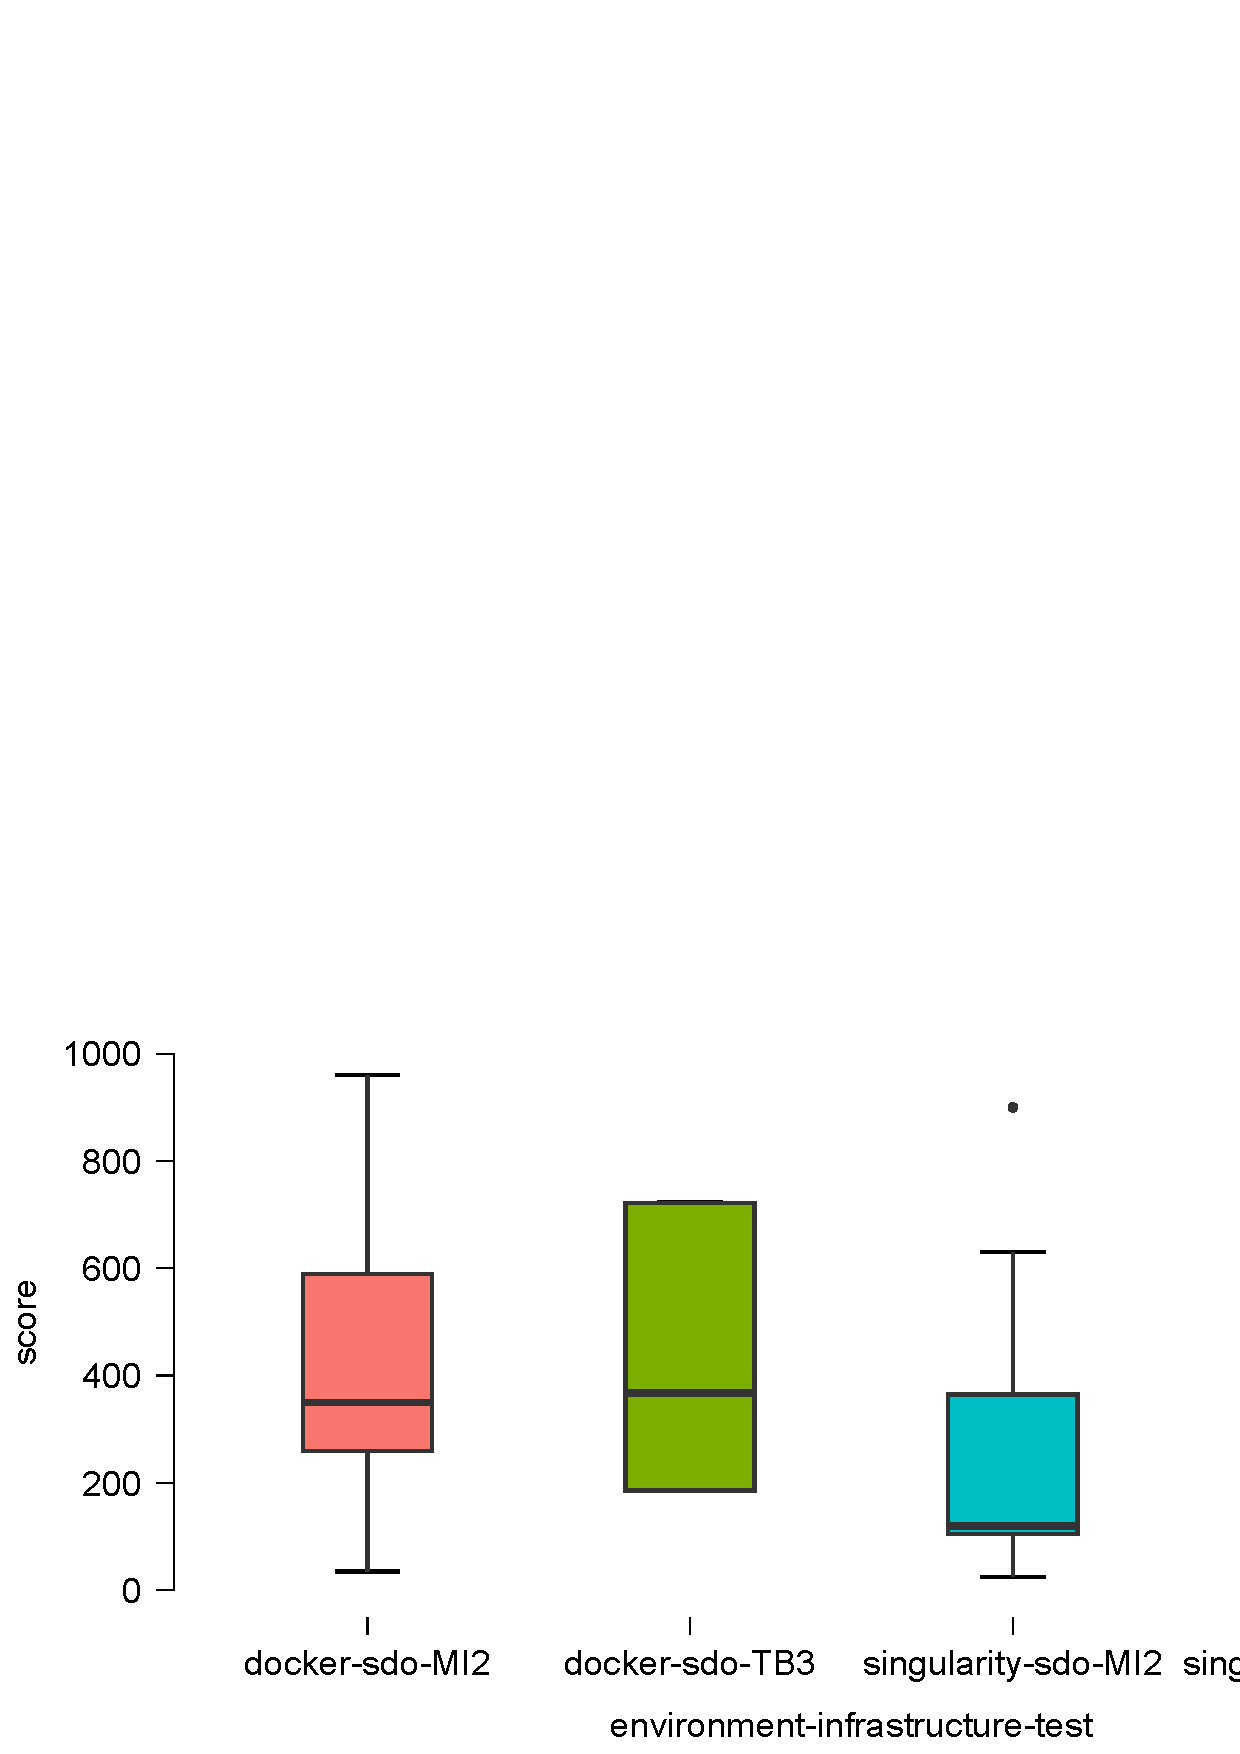
\includegraphics[width=\linewidth]{./figures/data/Boxplot_VAR_score_SPLIT_enviroment-infrastructure-test_FILTER_sdo.pdf}    }
    \caption{Comparison between sdo environments and fuzzing tests using the average score of all single-task runs.}
    \label{fig:Boxplot_score_sdo-evn-test}
\end{figure*}

%RAW DATA \url{https://github.com/b0rh/HOUSE/blob/master/B.OR/TB3-MI2_Robofuzz/Pruebas_enviroment-infrastructure-test%2Bsubtype/Pruebas_sdo-ALLTEST%2Bsubtype.csv}
    
  }

  \only<2>{
Performance comparison of single vs. parallel tasks.


%%Source: Pruebas_environment-infrastructure-test-subtype_score_hpc_uniq-paralell_sdo_uniq.csv

% 

%\begin{figure*}[ht!]
%%https://www.overleaf.com/learn/latex/Positioning_of_Figures
    \centerline{
\begin{tikzpicture}[scale=0.80]
\begin{axis}[
    symbolic x coords={sdo-MI2-2h,hpc-MI2-2h, hpc-MI2-2hx5, hpc-MI2-2hx10, hpc-MI2-2hx20, sdo-TB3-2h, hpc-TB3-2h, hpc-TB3-2hx5, hpc-TB3-2hx10, hpc-TB3-2hx20},
    bar width=10pt,
    xtick=data,
    x tick label style={rotate=90, anchor=east , inner sep=5pt}]
    \addplot[ybar,fill=blue!20] coordinates {
        (sdo-MI2-2h,0)  %% Workaround: para tener leyenda en el eje x
        (hpc-MI2-2h,0)  %% Workaround: para tener leyenda en el eje x
        (hpc-MI2-2hx5,340)
        (hpc-MI2-2hx10,710)
        (hpc-MI2-2hx20,980)
        (sdo-TB3-2h,0)  %% Workaround: para tener ejex en el eje x
        (hpc-TB3-2h,0)  %% Workaround: para tener ejex en el eje x
        (hpc-TB3-2hx5,183)
        (hpc-TB3-2hx10,353)
        (hpc-TB3-2hx20,494)
    };
     %\addlegendentry{Paralell task}
    \addplot[ybar,fill=red!20] coordinates {
        (sdo-MI2-2h,0)  %% Workaround: para tener leyenda en el eje x
        (hpc-MI2-2h,16.666666671)
        (sdo-TB3-2h,0)  %% Workaround: para tener ejex en el eje x
        (hpc-TB3-2h,96.333333331)
    };
    \addplot[ybar,fill=green!20] coordinates {
        (sdo-MI2-2h,395)
        (sdo-TB3-2h,367.6666667)
    };
    
    %\addlegendentry{Unique task}
    
\end{axis}
\end{tikzpicture}}
    % El contenido de legendbox se cambia en package.tex linea 55 donde se define el robustcommand usado para dibujarlo.
%    \caption{The diagram presents a comparison between: \legendbox{green} the average score of 2h single tasks using a standalone computer (sdo), \legendbox{red} the average score of 2h single tasks using the singularity environment in the HPC infrastructure, and \legendbox{blue} parallel tasks using the score accumulated by the n parallel jobs in the HPC.}
%    %\caption{Comparativa entre tareas paralelas  \legendbox{blue} usando el score acumulado por las n tareas paraleleas  y el socre medio de tareas unicas de 2h \legendbox{red}  usando el entorno singularity en la infraestructura de HPC. Y el score medio de 2h en tareas unicas \legendbox{green} usando sdo.}
%    \label{fig:Barplot_score_by_paralell-unique_hpc}
%\end{figure*}
  }

\end{frame}

\section{Conclusions}
%\frame{\sectionpage}
\begin{frame}{Conclusions}
\only<1>{
    \begin{itemize}
    \item High-Performance Computing improves fuzzing testing by providing computational resources, parallel processing, and advanced algorithms for complex systems.

\item Recent kernels outperform older ones due to container management improvements and processor vulnerability patches; parallelization reduces task completion time.
\end{itemize}
}

 \only<2>{

These are this work's three main contributions:
\begin{tcolorbox}[drop shadow southeast,
enhanced,colback=blue!5!white,colframe=Azuloscuro-cisis]

\begin{enumerate}
    \item Empirical evaluations that allow us to answer the hypothesis above.
    \item A set of publicly available Singularity containers deploying a ROS 2 fuzzer. 
    \item Lessons learned of using a SOTA fuzzer in an HPC environment. 
\end{enumerate}
\end{tcolorbox}
  }


\end{frame}


\section{Next steps}
%\frame{\sectionpage}
\begin{frame}{Next steps}
\begin{itemize}
    \item
Adapt completely HOUSE framework to robotic environments using ROS for decoupled deployment in HPC, improving fuzzying processes in multi-variable contexts.
\end{itemize}
\end{frame}



% DEMO %%%%%%%%%%%%%%%%%%%%%%%%%%%%%%%%%%%%%

\begin{frame}
%\begin{frame}[plain,standout]
\begin{center}
\vspace*{\stretch{1}}
{\centering\Huge\textcolor{black!50}{Demo time}\par}%
\vspace*{\stretch{1}}
\end{center}
    
\end{frame}

% PREGUNTAS %%%%%%%%%%%%%%%%%%%%%%%%%%%%%%%%%%%%%

\begin{frame}
%\begin{frame}[plain,standout]
\begin{center}
\vspace*{\stretch{1}}
{\centering\Huge\textcolor{black!50}{Thank you for your attention.}\par Do you have any questions?}%
\vspace*{\stretch{1}}
\end{center}
    
\end{frame}

%\titleframe
%\appendix

% REFERENCIAS %%%%%%%%%%%%%%%%%%%%%%%%%%%%%%%%%%%%%
%
%\begin{frame}[allowframebreaks]{References}
%
%    \bibliographystyle{spmpsci}
%    \bibliography{bibliography.bib}
%
%\end{frame}


\end{document}

